\chapter{Field-level inference}\label{ch:field-level}
\chapterstatus{written}{2026-11-14}

Field-level inference samples the joint posterior of the initial density field and the parameters given a tracer field, without
compressing the data into summary statistics \cite{JascheWandelt2013,Stadler2024}. \fml{} has a periodic framework (forward models,
likelihoods, adjoint gradients, exact linear references, MAP and Hamiltonian Monte Carlo), distributed versions on slabs and pencils, a
masked Cartesian survey layer, a differentiable particle-mesh forward model, and the original BAO prototype.

\begin{modulebox}{FieldLevel}
\nsp{FML::FIELDLEVEL::FRAMEWORK}: \file{FieldLevel/Framework.h} (\cls{Configuration}, \cls{Model}, \cls{Posterior}, \code{map},
\code{sample}, \code{linear_conditional}), \file{DistributedLinear.h}, \file{DistributedLPT.h}, \file{DistributedAssignment.h},
\file{SurveyLikelihood.h}, \file{ParticleMesh.h}, \file{ParticleMeshAdjoint.h}, \file{ParticleMeshPosterior.h},
\file{Checkpoint.h}, \file{SurveyCheckpoint.h}, \file{Frontend.h}; \nsp{FML::FIELDLEVEL}: \file{FieldLevelBAO.h}.\par
Documentation: \file{FieldLevel/docs/BAO.md}, \file{docs/FRAMEWORK.md}, \file{docs/SURVEY.md}, \file{docs/PARTICLE_MESH.md}, \file{docs/PM_ADJOINT.md},
\file{docs/PM_POSTERIOR.md}, \file{docs/KNOWN_ISSUES.md}. Tests and validation records in \file{FieldLevel/tests} and \file{FieldLevel/validation/survey}.
\end{modulebox}

\section{The probability model}\label{sec:fl-model}

The sampled field is a real white Gaussian vector $s$ on an $N^3$ grid with prior $-\ln p(s)=\frac12\sum s^2$; the linear field is
\begin{equation}
\delta_L(\bm k)=\sqrt{\frac{P(k;\theta)N^3}{V}}\,s(\bm k),\qquad0<k<k_{\rm init},
\end{equation}
(\code{r2c} divides by $N^3$, so $\langle|\delta_{\bm k}|^2\rangle=P/V$), with the spectrum and its parameter derivatives supplied by a callback.
The scalar parameters (spectrum parameters, bias $b_1$, $b_2$, $b_{s^2}$, $b_{\nabla^2}$, $\ln P_\epsilon$) have Gaussian or uniform priors. The Gaussian
field likelihood over the full Hermitian set of modes below $k_{\rm like}$ is
\begin{equation}
U_{\rm data}=\frac12\sum_{\bm k}\left[\frac{|\delta^{\rm pred}_{\bm k}-d_{\bm k}|^2}{P_\epsilon/V}+\ln\frac{P_\epsilon}{V}\right],
\end{equation}
(the normalisation is kept when the noise is sampled).

\section{Forward models and adjoints}\label{sec:fl-forward}

\begin{itemize}
\item \code{Linear}: $\delta^{\rm pred}=(b_1+f\mu^2)\delta_L$.
\item \code{Zeldovich} and \code{LPT2}: one particle per cell displaced by 1LPT or 2LPT (\cref{ch:lpt}, \cite{Crocce2006}), carrying the Lagrangian bias weight
      $1+(b_1-1)\delta_b+b_2(\delta_b^2-\langle\delta_b^2\rangle)+b_{s^2}(s^2-\langle s^2\rangle)+b_{\nabla^2}\nabla^2\delta_b$ of the field smoothed at
      $k_{\rm bias}$, with plane-parallel RSD $x_z\mathrel{+}=f\Psi^{(1)}_z+2f\Psi^{(2)}_z$, assigned to a finer density grid with a smooth compact kernel whose
      Fourier transform is divided out (the modes equal the direct Fourier sum over particles to $3\times10^{-5}$) and a differentiable gradient (CIC would
      respond non-smoothly to displacements of particles on nodes).
\item \code{ParticleMesh}: a periodic PM evolution in a flat $\Lambda$CDM background from Zel'dovich initial conditions, with a discrete adjoint using bounded
      in-memory checkpoints and recomputation.
\end{itemize}
The gradient of $U$ is computed with hand-written adjoints at about twice the cost of a forward model: the residual on the modes, back through the assignment
(the gradient of the kernel for the positions, the kernel for the weights), the RSD map, 2LPT and the bias operators to $\delta_L$, and to $s$ and $\theta$. Every
adjoint is checked against finite differences.

\begin{figure}[htbp]
\centering
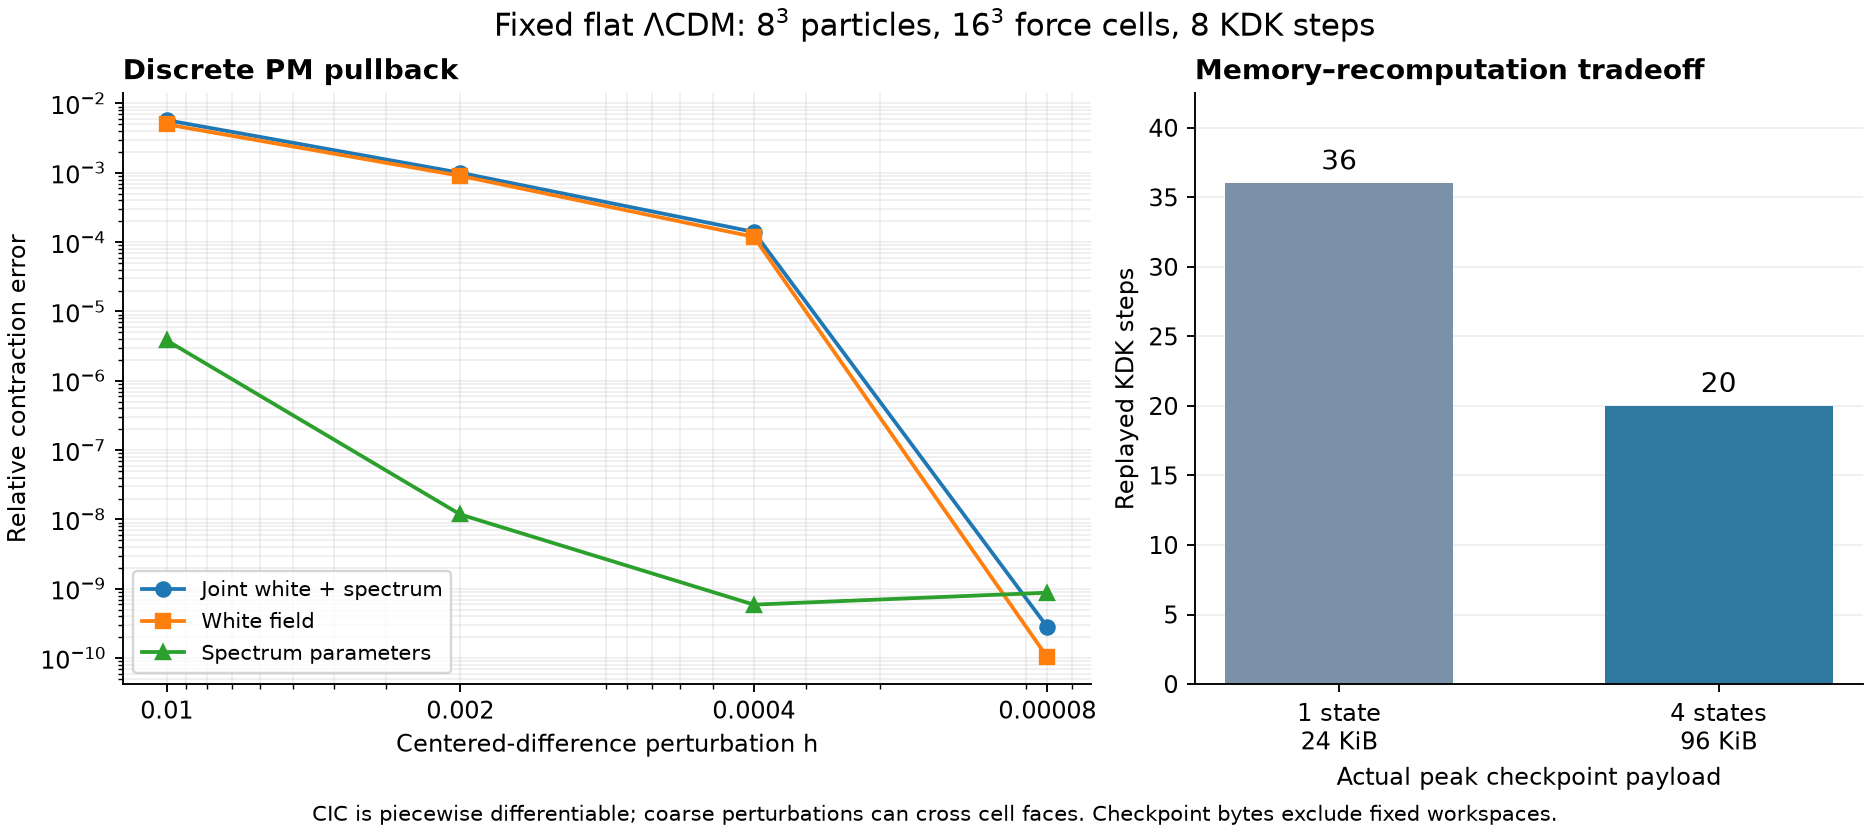
\includegraphics[width=0.9\textwidth]{fieldlevel_pm_adjoint}
\caption{The discrete adjoint of the particle-mesh forward model ($8^3$ particles, $16^3$ force cells, 8 kick-drift-kick steps): the relative
error of the reverse-mode contraction against centred finite differences as the step $h$ decreases, and the number of replayed steps for
one or four stored states (\file{FieldLevel/tests/figures}).}
\label{fig:fl-pm-adjoint}
\end{figure}


\section{Inference}\label{sec:fl-inference}

For linear evolution at fixed parameters the posterior of the field is Gaussian: \code{linear_conditional} gives the exact mean, the Fourier covariance and the
field-marginalised likelihood, used as references. \code{map} finds the maximum a posteriori field (and optionally parameters) with a Fourier preconditioner and
line search. \code{sample} uses the Hamiltonian Monte Carlo of \cref{ch:sampling-fitting} \cite{Duane1987,Neal2011} with a Fourier-diagonal mass for the field (the
linear Hessian $1+b^2P/P_\epsilon$, frozen at the initial parameters), adapted masses for the scalars, and a callback to stream field samples (initial and matter
densities, displacements, velocities). Partial centring of the field, $s_k=(T(\theta_{\rm ref})/T(\theta))^cx_k$ with $c=S/(S+N)$ per mode, decorrelates the field and
the spectrum parameters (the BAO autocorrelation time drops from $\sim13$ to $\sim3$).

\paragraph*{Distribution and restart.} The distributed backends run the linear, 1LPT and 2LPT models, their adjoints, exact conditionals, MAP and HMC over MPI on slab
or pencil grids, with particle/mesh communication for the assignment (\cref{ch:mass-assignment}); checkpoints save the complete HMC and adaptation state with an identity
fingerprint of the backend and grid partition for exact same-layout restarts.

\paragraph*{Surveys.} \file{SurveyLikelihood.h} adds a masked Cartesian observation on the initial mesh: a window with observed flags and selection per cell, the model's
Fourier modes synthesised to real space, and either a Gaussian field likelihood or a Poisson count likelihood with a positive log-link,
$\ln\lambda_i=\ln E_i+\ln S_i+\delta_i-{\rm offset}$, $U_i=\lambda_i-n_i\ln\lambda_i+\ln n_i!$, both with MPI adjoints.

\section{BAO application}\label{sec:fl-bao}

\file{FieldLevelBAO.h} is a prototype of field-level BAO inference \cite{Babic2024}: the BAO scale $\beta=r_{\rm BAO}/r_{\rm fid}$ is sampled with the initial field, the
spectrum being a no-wiggle Eisenstein--Hu shape times $1+A\sin(k\beta r_{\rm fid}+\phi)e^{-k/k_d}$, with linear, 1LPT and 2LPT+bias+RSD forward models (bias, growth
rate and noise fixed). For the linear model the marginal posterior of $\beta$ is known exactly and HMC agrees with it ($1.0232\pm0.0333$ exact, $1.0221\pm0.0330$ HMC on
$32^3$, $k_{\max}=0.095\hMpc$).

\begin{figure}[htbp]
\centering
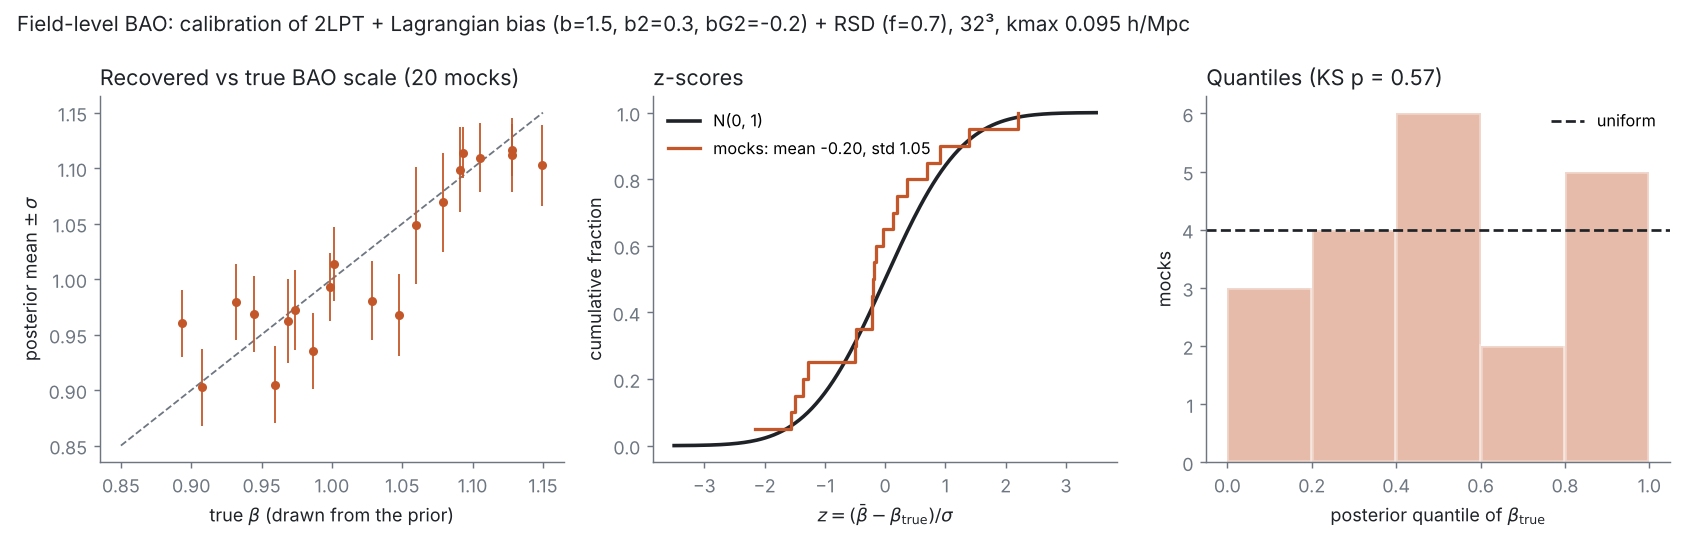
\includegraphics[width=\textwidth]{fieldlevel_bao_calibration}
\caption{Simulation-based calibration of field-level BAO inference with 2LPT, Lagrangian bias ($b=1.5$, $b_2=0.3$, $b_{\mathcal G_2}=-0.2$) and
RSD ($f=0.7$) on $32^3$, $k_{\max}=0.095\hMpc$ (20 mocks, $\beta_{\rm true}$ drawn from the prior): the recovered scale, the $z$-scores against
$\mathcal N(0,1)$ and the posterior quantiles of the true value (\file{FieldLevel/docs/images/calibration.png}).}
\label{fig:fl-calibration}
\end{figure}


\begin{validation}[Validation: field level]
Adjoint gradients against finite differences for all models (relative $\sim10^{-8}$); 2LPT of two orthogonal plane waves against the analytic displacement to $10^{-16}$;
the 2LPT+bias+RSD prediction equals $(b+f\mu^2)\delta_L$ in the linear regime to 0.3\%; mock $\chi^2$ equal to the number of modes. Simulation-based calibration
\cite{Talts2018}: for linear, 1LPT and the full 2LPT+bias+RSD model (20--30 mocks each) $z=(\bar\beta-\beta_{\rm true})/\sigma$ has mean consistent with zero and unit width and
the posterior quantiles are uniform (KS $p=0.57$--0.85). The distributed backends agree with the serial ones for any decomposition; the survey layer is validated with
dispersed 2LPT chains against exact active-mode and masked linear-Gaussian references (\file{FieldLevel/validation/survey}). These checks establish the numerics and sampler, not
nonlinear accuracy against simulations or a production survey analysis.
\end{validation}
